\section{Introduction}

Static analysis of code is one of the most effective ways to avoid defects in software, and, when security is a concern, is simply essential.  Static analysis can find problems that are extremely hard to detect by testing, when the inputs triggering a bug are hard to find.  Static analysis is also often more efficient than testing; a bug that takes a fuzzer like AFL days to find may be immediately identified by a good static analysis tool.

Users of static analysis tools often wonder which of multiple tools available for a programming language are most effective, and, when using more than one tool is an option, which is often the case, how much tools overlap in their results.  Given the human effort required to read static analysis results, the latter can be an important question.  If two tools find substantially different bugs, it is important to use both tools \cite{AllBugs}.  On the other hand, if two tools are very similar in what they detect, the effort to configure and use both, and especially of wading through duplicate results, may not be a good use of time.  Developers of static analysis tools also want to be able to compare their tools to others targeting the same domain, in order to see what detection methods or tweaks to precision/soundness trade-offs they might want to imitate.  Unfortunately, comparing static analysis tools is hard, and would seem to require vast manual effort to inspect findings and determine ground truth on a scale that would provide statistical confidence.

Differential testing \cite{Differential,ICSEDiff,csmith} is a popular approach to comparing multiple software systems offering similar functionality, but the wide divergence of possible trade-offs, analysis focuses, and the prevalence of false positives in almost all analysis results makes na\"ive differential testing not applicable to static analysis tools \cite{regehrRandom}.

Mutation analysis\cite{jia2011analysis,demillo1978hints,budd1980theoretical} uses small syntactic changes to a program to introduce synthetic ``faults,'' under the assumption that if the original version of a program is mostly correct, such changes will often introduce a fault.  For the most part, mutation analysis has been used to evaluate test suites by computing a mutation score, the fraction of mutants the suite detects, or ``kills''.  Most such use has been in research efforts, rather than practical testing efforts, though there has been sporadic use by interested developers.
Groce et al. \cite{groce2015verified,groce2018verified} proposed examining individual mutants that survive a rigorous testing and verification effort to detect and correct weaknesses in such efforts.  The approach was able to expose bugs in a heavily-tested module of the Linux kernel \cite{mutKernel} and a widely used Python file system.  Recently, mutation analysis has been adopted in industrial settings, though not for actual examination of all surviving mutants \cite{MutGoogle,ivankovic2018industrial}, due to scale.

Combining a differential approach and mutation analysis offers a novel way to compare static analysis tools, one useful to users wishing to select a good tool or set of tools, to researchers interested in the impact of precision/soundness trade-offs or different intermediate languages, and to developers of static analysis tools hoping to improve their tools by examining missed faults.

\subsection{Differential Mutation Analysis}

We can say that a static analysis tool kills a mutant when the \emph{number of warnings or errors}, which we call \emph{findings}, that are not informational or optimization related, i.e., that are \emph{fault-related}, produced with respect to the code \emph{increases} for the mutated version, compared to the original code. That is, when the tool ``finds more bugs'' for the mutated code.  This difference may be most easily interpreted when the original code produces no findings; we call such code \emph{clean}. For non-clean code, a tool conceivably could detect the mutant, but only change a previously generated finding, not add an additional finding, leading to an underestimate of effectiveness.  However, even for non-clean code, \emph{most detected mutants should produce a new warning}.  We count findings, rather than consider their location or type, because some mutants cause a fault at a far-removed location.  Forcing tools to produce an \emph{additonal} warning is a conservative and automatable estimate of mutant detection.

The value of the differential comparison lies in a few key points.  First, this is a measure that does not reward a tool that produces too many false positives.  The tool cannot simply flag all code as having a problem or it will perform poorly at the task of \emph{distinguishing} the mutated code from non-mutated, and presumably at least \emph{more} correct, code.  Based on verification and testing uses of mutation, it is safe to say that usually at minimum 40\%, often 50-60\%, and frequently up to 80\%+ \cite{mutKernel,groce2018verified,le2014mucheck}, of mutants are not semantically equivalent to the original code \cite{TCE,impactEquiv,smith2009should}, so the task presented to a static analysis tool is simply the core functionality of static analysis \emph{to distinguish faulty from correct code without execution}.  Obviously, many faults cannot be identified statically without a complete specification, or without unreasonable analysis cost and precision, but the measure of performance here is \emph{relative} to other tools applied to the same code; this is primarily a \emph{differential} approach.  In other words, a key notion is that while most mutants cannot be detected statically, the ones that are tend to be \emph{true positives}: \emph{if} they were real code changes, they would be faults.  We manually confirmed that for most mutants in our experiments where any tool detected the mutant (and at least one tool did not), the changes were indeed ones that would be real faults if present in the code.

Second, and critically, this is an \emph{automatable} method that can provide an evaluation of static analysis tools over a large number of target source code files, without requiring human effort to classify results as real bugs or false positives.  It is not clear that any other fully automatic method is competitively meaningful; it is possible that methods based on code changes from version control provide some of the same benefits, but these require classification of changes into bug-fixes and non-bug-fixes, and of course require version control history.  Also, history-based methods will be biased towards precisely those faults humans or tools already in use were able to detect and fix.  Rather than the hundreds \cite{just2014defects4j} or at most few thousand of faults \cite{BugSwarm} in benchmark defect sets, our approach enables the use of \emph{many tens of thousands} of hypothetical faults.

It is the combination of differential comparison and mutation that is key.  Differential comparison of tools, as noted above, is not really meaningful, without additional effort; na\"ive methods simply will not work \cite{regehrRandom}.  Consider a comparison of the number of findings between two tools over a single program, or over a large set of programs.  If one tool emits more warnings and errors than another, it may mean that the tool is more effective at finding bugs; but it may also mean that it has a higher false positive rate.  Without human examination of the individual findings, it is impossible to be sure, or even (in cases where the tools are reasonably comparable) to make an informed guess.  Using mutants, however, provides a foreground to compare to this background.  In particular, for a large set of programs, the most informative result will be when 1) tool A reports fewer findings on average than tool B over the un-mutated programs but 2) tool A also detects more mutants.  This is strong evidence that A is simply better all-around than B; it likely has a lower false positive rate \emph{and} a lower false negative rate.  While it is not proof of this claim, it is hard to construct another plausible explanation for reporting \emph{fewer} findings on un-mutated code while still detecting \emph{more} mutants.  Other than having better precision and recall, how else could a tool effectively distinguish mutated from un-mutated code?

We can quantitatively express the relationship between detecting mutants and findings for the original program.  Since we are comparing over the same program or set of programs, we simply divide the mean \emph{mutation score} ($\frac{|\mathit{killed}|}{|\mathit{mutants}|}$, the ratio of killed mutants to all mutants) by the mean number of findings.  This \emph {mutant ratio} tells us about the ability of a tool to produce findings \emph{for mutants}, relative to its tendency to produce findings in general, (per line of code, per source file, etc.).  If a tool has a tendency to produce large numbers of findings compared to other tools, and this is paired with a tendency to detect most mutants, then the tool will not be penalized for producing many findings.  Assuming that real faults are relatively rare in the original, un-mutated code, the best result and best mutant ratio will be for a tool that produces comparatively few findings for un-mutated code, but detects a larger portion of mutants than other tools; the worst result will be a tool that produces lots of findings, but detects few mutants.  We will actually see some examples of the worst case in our results for real tools.

\begin{figure}
  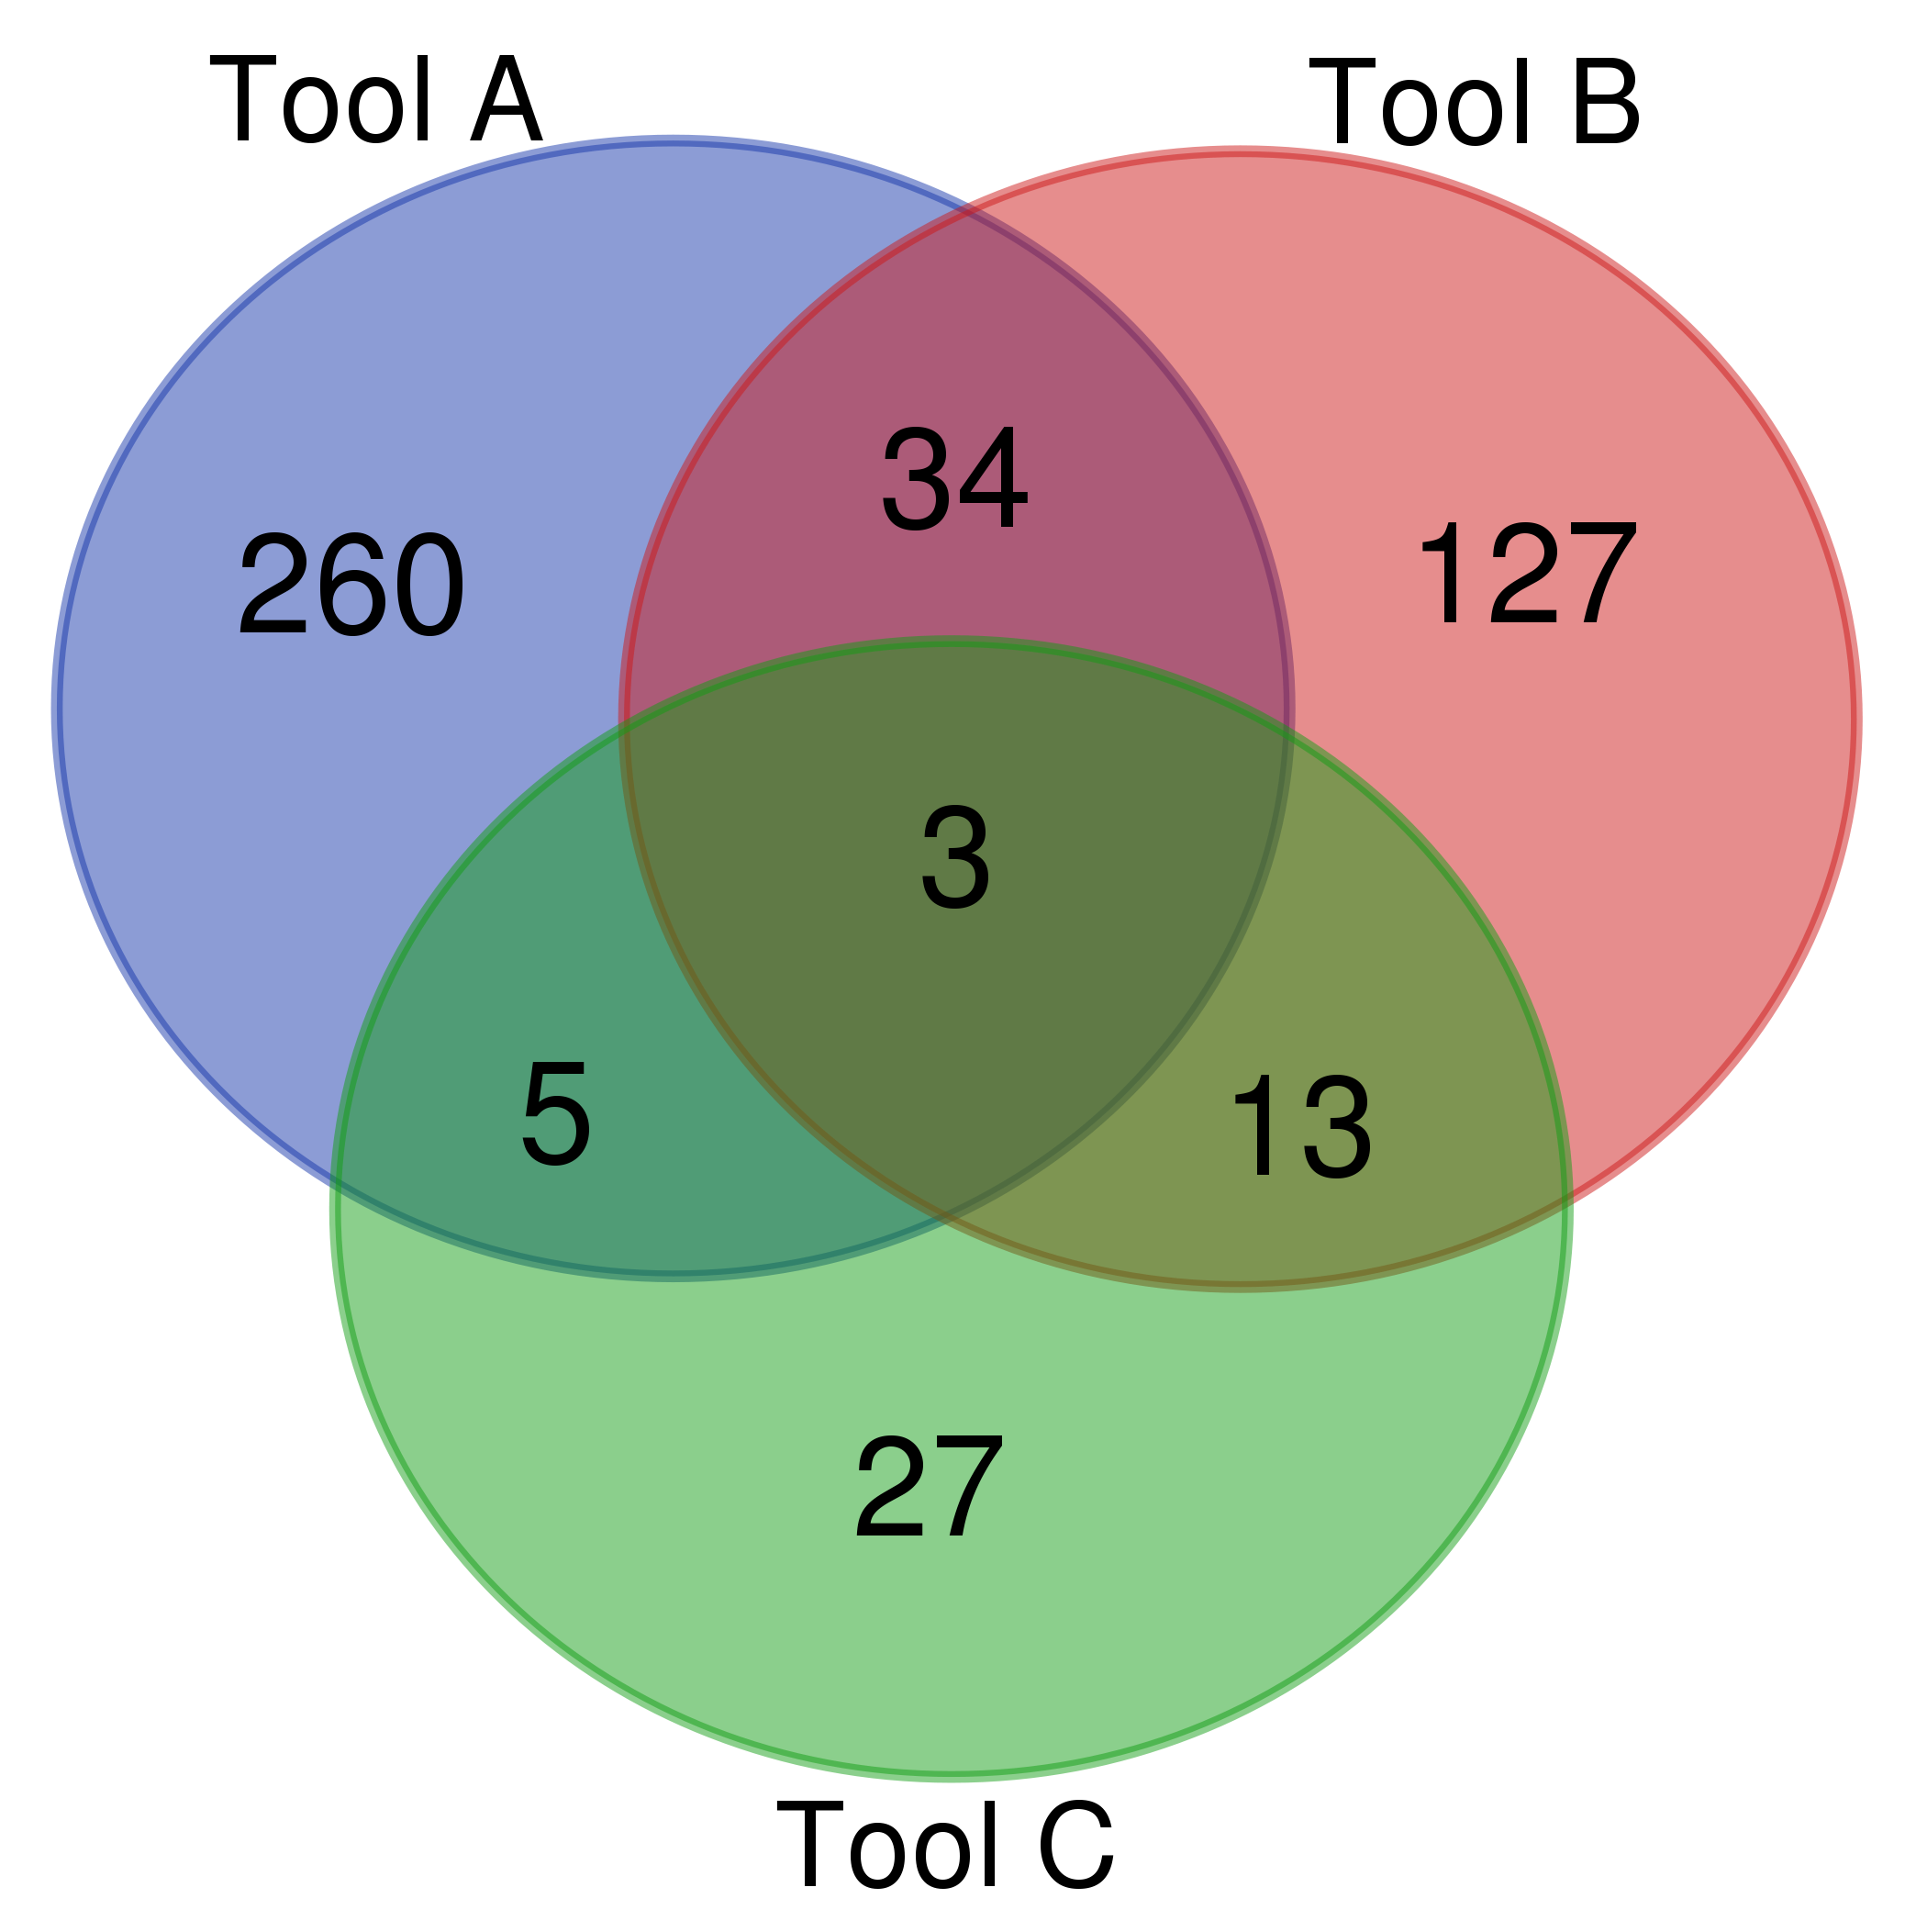
\includegraphics[width=0.4\columnwidth]{example.png}
  \caption{Mutants killed by three static analysis tools.}
  \label{fig:examplevenn}
\end{figure}

Finally, even when tools have similar quantitative results, including similar ratios, examining individual mutants killed by one tool but not by another allows us to understand strengths and weaknesses of the tools, in a context that makes comprehending the cause of the detection, or lack of it, easy: the difference between the un-mutated code and mutated code will always be small and relatively simple.  Moreover, simply looking at how much two tools agree on mutants can answer the question of a user of static analysis tools: given that I am using tool A, would adding tool B be likely to add enough new, interesting results to make it worth my time to examine its output?  When one tool subsumes another in terms of mutants, it can be very clear that the tool whose killed mutants are all killed by another tool is likely strictly inferior.  Interested users, e.g. security analysts, can inspect the differences to get an idea of the particular cases when a tool might be most effective, but a more typical user can simply look at a Venn diagram of kills like that shown in Figure \ref{fig:examplevenn}.  Assume that tools A, B, and C all produce very similar numbers of findings for un-mutated code, and have similar execution times.  Tool A is likely the most important tool to make use of; it detected more mutants than any other tool, and more than twice as many mutants were killed by A alone than by B alone.  However, also running tool B is probably a very good idea, assuming, e.g., it is not a very expensive commercial tool.  B does not do as well as A, but it is the only tool that detects a large number of mutants, and most mutants it detects are unique to it.  Finally, Tool C \emph{may} not be worth running; recall that it produces a similar number of findings to A and B on the un-mutated code, so it is notably bad at detecting faults, at least ones that look like mutants.  It might be a good idea to just look at the 27 mutants detected by C alone:  if they represent an important class of potential problems (perhaps C specialized in detecting potentially non-terminating loops), then C might be useful, but if the first few mutants inspected are false positives, then C is likely not useful.

Comparing mutant results also leads to the idea of \emph{improving} static analysis tools by examining mutants detected by another tool, and thus known to be in-principle detectable, but not detected by the tool to be improved.  Improving tools by adding detectors is useful because, even if all tools had the same set of detectors, they would not all report the same bugs; different choices in intermediate language and tradeoffs made to avoid false positives may make the use of multiple tools with similar detectors essential for thorough analysis.  And if one tool simply has a superior engine, it is beneficial to users that the ``best'' tool incorporate \emph{all} detection rules.

Of course, any faults in code, not just mutants, could serve this purpose.  But, again, the automatic nature of mutation generation, and the presumption that the mutation is indeed a fault, is useful.  Moreover, because mutants follow syntactic patterns, searching for similar mutants/faults the tool to be improved does not detect is much easier than with arbitrary faults, and can be partly automated.   However, as with efforts to improve test suites, manually searching through all mutants can be an onerous task, especially for large-scale evaluations.  We therefore also introduce the idea of prioritizing mutants, using a Furthest-Point-First \cite{Gonzalez} algorithm and distance metric inspired by previous work on helping developers sort through failing test cases to find distinct faults \cite{PLDI13,distMut}, to help static analysis tool developers find interesting patterns without wading through numerous uninteresting mutants.

A general objection to our approach is that mutants may differ substantially from ``real'' faults, in some way.  This is certainly true, in a sense \cite{GopinathMutants}, but for static analysis purposes we believe it does not matter.   The real risk is that some mutation operators align with patterns a particular tool identifies, biasing the evaluation in favor of that tool.  Such faults may be dis-proportionately present in mutants vs. real code.  However, we consider this unlikely.  The vast majority of applied mutation operations for all of our experiments were highly generic, and do not plausibly represent a pattern in which some tool might specialize.  Statement deletions leave no ``trace'' for a tool to match against, but only an omission.  Changing arithmetic and comparison operators and numeric constants (incrementing, decrementing, or changing to 0 or 1) account for most of the non-statement-deletion mutants.  We cannot see how any tool could have a useful detection rule that looks for these kinds of changes: a tool obviously could not flag all instances of 0 and 1 constants, or of addition, and remain a useful tool.  Finally, many mutants, though far fewer than in the previously noted categories, add {\tt break} or {\tt continue} statements.  Again, we do not see how a tool could take advantage of this without either genuinely understanding likely-bad control flow patterns, in which case, we think it ``deserves'' to kill more mutants, or flagging so many legitimate uses of {\tt break} and {\tt continue} in un-mutated code that it would have a bad mutant ratio, due to producing more warnings than other tools. 

\subsection{A Simple Example}

\begin{figure}
{\scriptsize
\begin{code}
contract SimpleStorage \{
    uint storedData;

    function set(uint x) public \{
        storedData = x;
    \}

    function get() public view returns (uint) \{
        return storedData;
    \}
  \}
\end{code}
}
\caption{A simple example Solidity smart contract}
\label{fig:sol424intro}
\end{figure}

Consider the code in Figure \ref{fig:sol424intro} \cite{solintro}.  The Universal Mutator tool \cite{universalmutator,regexpMut}, which has been extensively tuned for Solidity's grammar (though not to target any particular vulnerabilities), and is the only smart contract mutation tool referenced in the Solidity documentation (\url{https://solidity.readthedocs.io/en/v0.5.12/resources.html}), produces seven valid, non-redundant (by Trivial Compiler Equivalence \cite{TCE}) mutants for this trivial example code.  Both the public version of Slither \cite{slither} and SmartCheck \cite{smartcheck} produce a small number (three and two, respectively) of low-severity, informational, warnings for this code.  Both tools also detect (by increasing the number of warnings produced) four of the seven mutants.  However, only one of the mutants detected is common to both tools: both tools detect changing the {\tt return} statement in the {\tt get} function to a call to {\tt selfdestruct} the smart contract, deleting it.  Slither, but not SmartCheck, also detects replacing the assignment of {\tt storedData} in {\tt set} with either a {\tt selfdestruct} or {\tt revert}, or simply removing it altogether.  SmartCheck, on the other hand, detects removing the {\tt return} in {\tt get} or replacing it with a {\tt revert}, or removing the {\tt public} visibility modifier for {\tt get} \footnote{Slither's ``missing return'' detector is only available in the private version of slither, or through the {\tt crytic} service provided by Trail of Bits.}.  If we restrict our analysis to findings with a severity greater than informational, SmartCheck detects no mutants of the contract, while Slither still reports that some mutants \emph{allow an arbitrary caller to cause the contract to destroy itself}.  This simple example shows how our approach works on a small scale.  Using large numbers of larger, more realistic contracts makes it possible to extract the same kind of information, on a much larger scale.  Prioritization of mutants is not very useful here (ranking three mutants saves little effort), so we will show the utility of that idea in our full Solidity results.

\subsection{Contributions}

This paper offers the following contributions:

\begin{itemize}[labelsep=3pt,leftmargin=12pt]
\item We propose a differential approach to comparing static analysis tools based on the insight that program mutants provide an automated source of simple, easy-to-understand program changes that are likely faults.
\item We propose a definition of mutant killing for static analysis.
\item We introduce a simple scheme for prioritizing mutants that helps users understand and use the results of analysis.
\item We apply our method to an extensive, in-depth comparison of three Solidity smart contract analysis tools, and show how prioritization allowed us to easily identify (and build) three new detectors for the most effective of these tools.
\item We further provide results for comparisons of popular Java and Python static analysis tools, showing the general usefulness of our methods, and giving a new picture of the comparative effectiveness of these tools.
\end{itemize}

The Solidity, Java, and Python case studies also serve to answer a set of research questions investigating the utility of our approach, and provide basic evidence that it provides actionable, non-obvious information that is otherwise difficult to produce.  While there are certainly limitations to using differential mutation analysis to compare and extend static analysis tools, the method scales to basing comparisons on large numbers of real software source files and very large numbers of faults, but still has some of the advantages of humans establishing ground truth for tool findings.